% Session 3 -- the bulk-boundary correspondence: an integer that has to jump
% Placement: sec. "What topology means for a Hamiltonian", after the
% interpolating-Hamiltonian paragraph.
% Rendered by figures/blender/s03f02_bulkboundary.py, labels in figures/overlays/s03f02_bulkboundary.tex.
\begin{aqmfigure}{fig:s03:bulkboundary}{The bulk-boundary correspondence, as an argument about an
integer. A Hamiltonian changes slowly in space from $H_1$ on the left to $H_2$ on the right, which
is the color of the backdrop. In the top row, the Chern number is an integer, so it cannot change
continuously from $C_1=1$ to $C_2=0$ and it can only jump. In the middle row, a jump is only allowed
where the quantization argument itself fails, which is where the gap closes, so the local gap must
go to zero somewhere in the interface region, at the cross. This is drawn schematically, in the
local-gap approximation. In the bottom row, the state that appears there is a gapless state bound to
the interface. This argument does not use any detail of how the interface is built, and only $C_1$
and $C_2$ enter, which is why the edge state survives rough boundaries and impurities. If we take
$H_2$ to be the vacuum, $C_2=0$, we obtain the chiral edge state of figure~\ref{fig:s03:chiraledge}
from a completely general argument.}
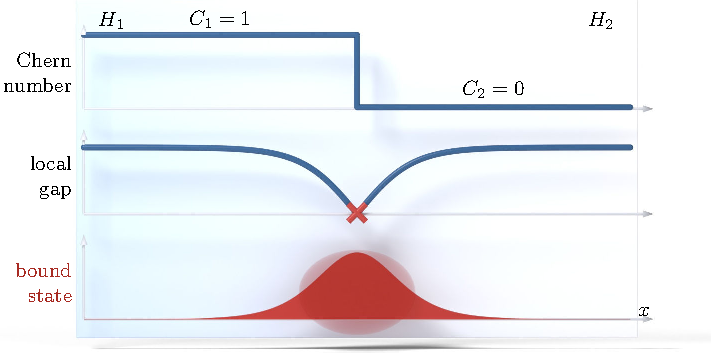
\includegraphics{figures/pdf/s03f02_bulkboundary.pdf}
\end{aqmfigure}
